\chapter{Additional Qualitative Results}
\section{BDD-Inpainting}
\Cref{fig:bus} and \Cref{fig:taxi} show additional results on tasks from the BDD-Inpainting test set. 
\begin{figure*}[h]
\begin{center}
    \centering
    \captionsetup{type=figure}
    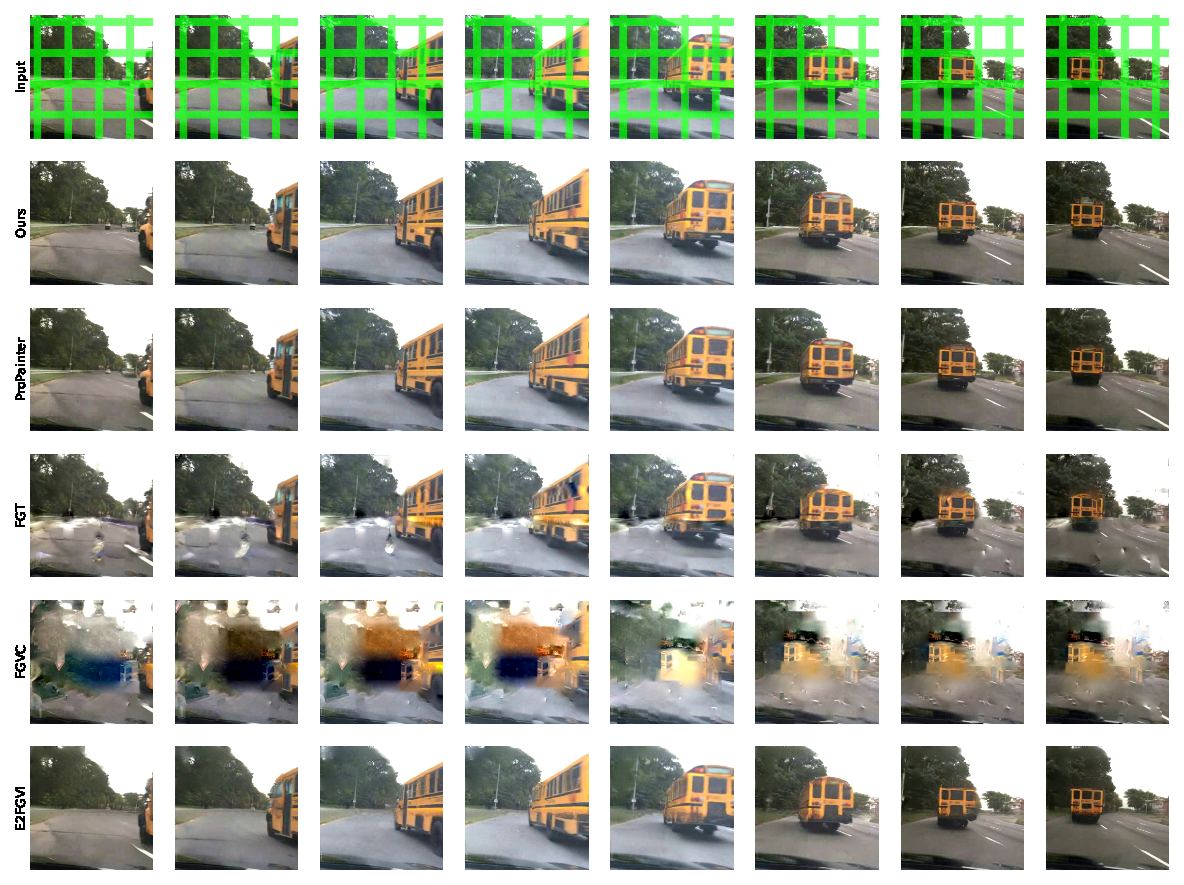
\includegraphics[width=\linewidth]{figures/additional-samples/bus_all.pdf}
    \caption[Qualitative results from our method and all competing methods on an example from the BDD-Inpainting-Blobs test set.]{Qualitative results from our method and all the competing methods we compared to quantitatively on an example from the BDD-Inpainting test set. We note that, in the presence of small masks, the qualitative differences are less pronounced between our method and the best-performing benchmarks, like since information in neighbouring frames can more easily be exploited. For our method we use the Improved AR w/ Far Future sampling scheme.}
    \label{fig:bus}
\end{center}
\end{figure*}



\begin{figure*}[h]
\begin{center}
    \centering
    \captionsetup{type=figure}
    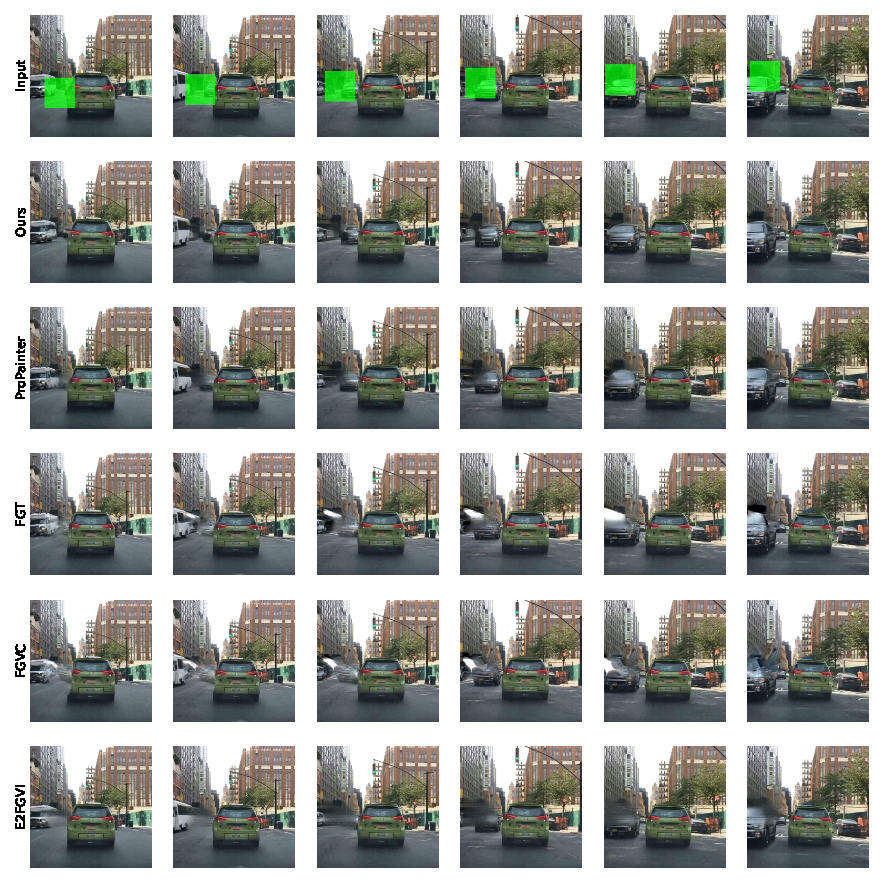
\includegraphics[width=\linewidth]{figures/additional-samples/taxi_all.pdf}
    \caption[Qualitative results from our method and all competing methods on an example from the BDD-Inpainting test set.]{Qualitative results from our method and all the competing methods we compared to quantitatively on an example from the BDD-Inpainting test set. Again, for our method we use the Improved AR w/ Far Future sampling scheme. In this video the vehicle passing in the left-hand lane is only ever partially visible, causing other methods to produce blurry results. }
    \label{fig:taxi}
\end{center}
\end{figure*}
\section{Traffic-Scenes}
\Cref{fig:ts1} and \Cref{fig:ts2} show additional results on tasks from the Traffic-Scenes training set.

\begin{figure*}[h]
\begin{center}
    \centering
    \captionsetup{type=figure}
    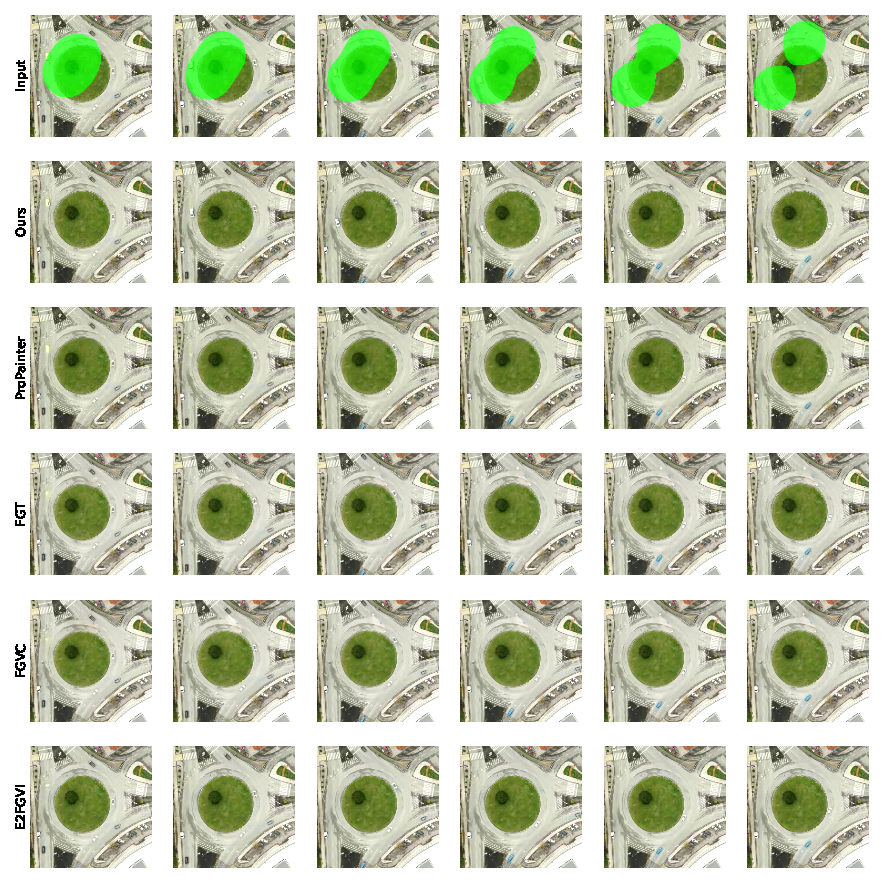
\includegraphics[width=\linewidth]{figures/additional-samples/ts1.pdf}
    \caption[Qualitative results from our method and all competing methods on an example from the Traffic-Scenes test set.]{Qualitative results from our method and all the competing methods we compared to quantitatively on an example from the Traffic-Scenes test set. For our method we use the Hierarchy-2 sampling scheme. For our method the two occluded vehicles are inpainted with continuous trajectories; for all other methods the vehicles disappear while they are occluded.} 
    \label{fig:ts1}
\end{center}
\end{figure*}

\begin{figure*}[h]
\begin{center}
    \centering
    \captionsetup{type=figure}
    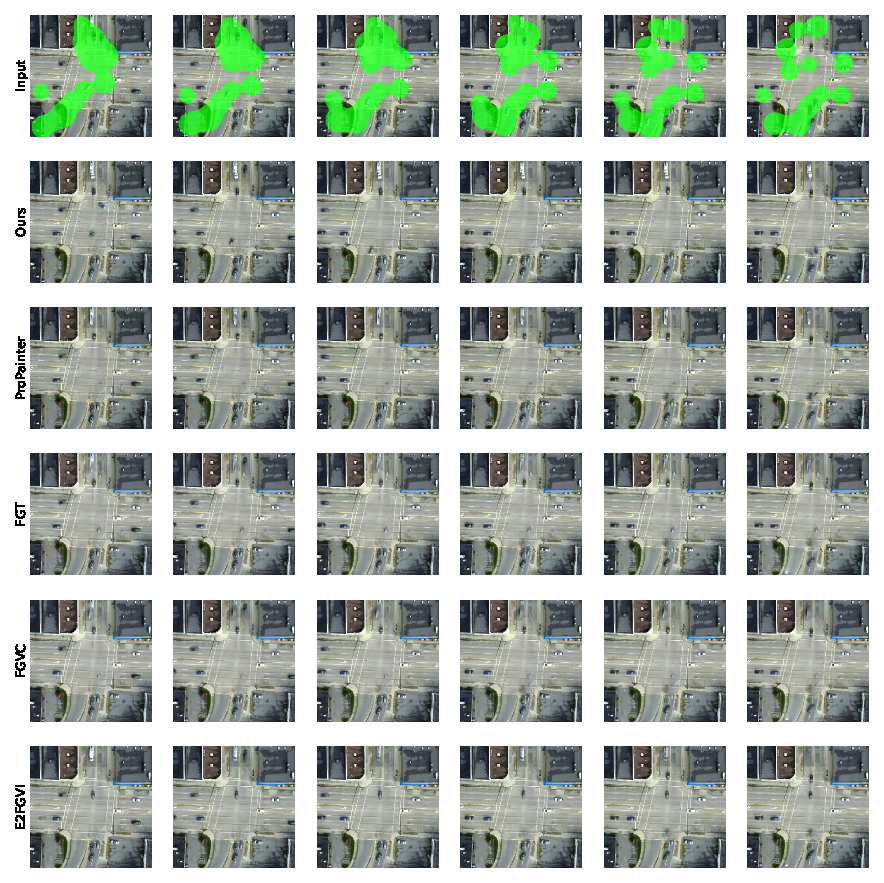
\includegraphics[width=\linewidth]{figures/additional-samples/ts2.pdf}
    \caption[Further qualitative results from our method and all competing methods on another example from the Traffic-Scenes test set.]{Further qualitative results from our method and all the competing methods we compared to quantitatively on an example from the Traffic-Scenes test set. In the ground truth for this example, in the first frame there is a vehicle making a left hand turn towards the bottom of the image that is occluded until it briefly emerges many frames later. Our model is able to initialize a vehicle in the inpainting and complete a trajectory which is consistent with the exit point for the vehicle. In all other methods the vehicle appears suddenly. } 
    \label{fig:ts2}
\end{center}
\end{figure*}

\section{Inpainting-Cars}
\Cref{fig:extra-cars} shows additional results on tasks from the Traffic-Scenes training set.

\begin{figure}[t!]
    \centering
    \begin{subfigure}[t]{\textwidth}
        \centering
        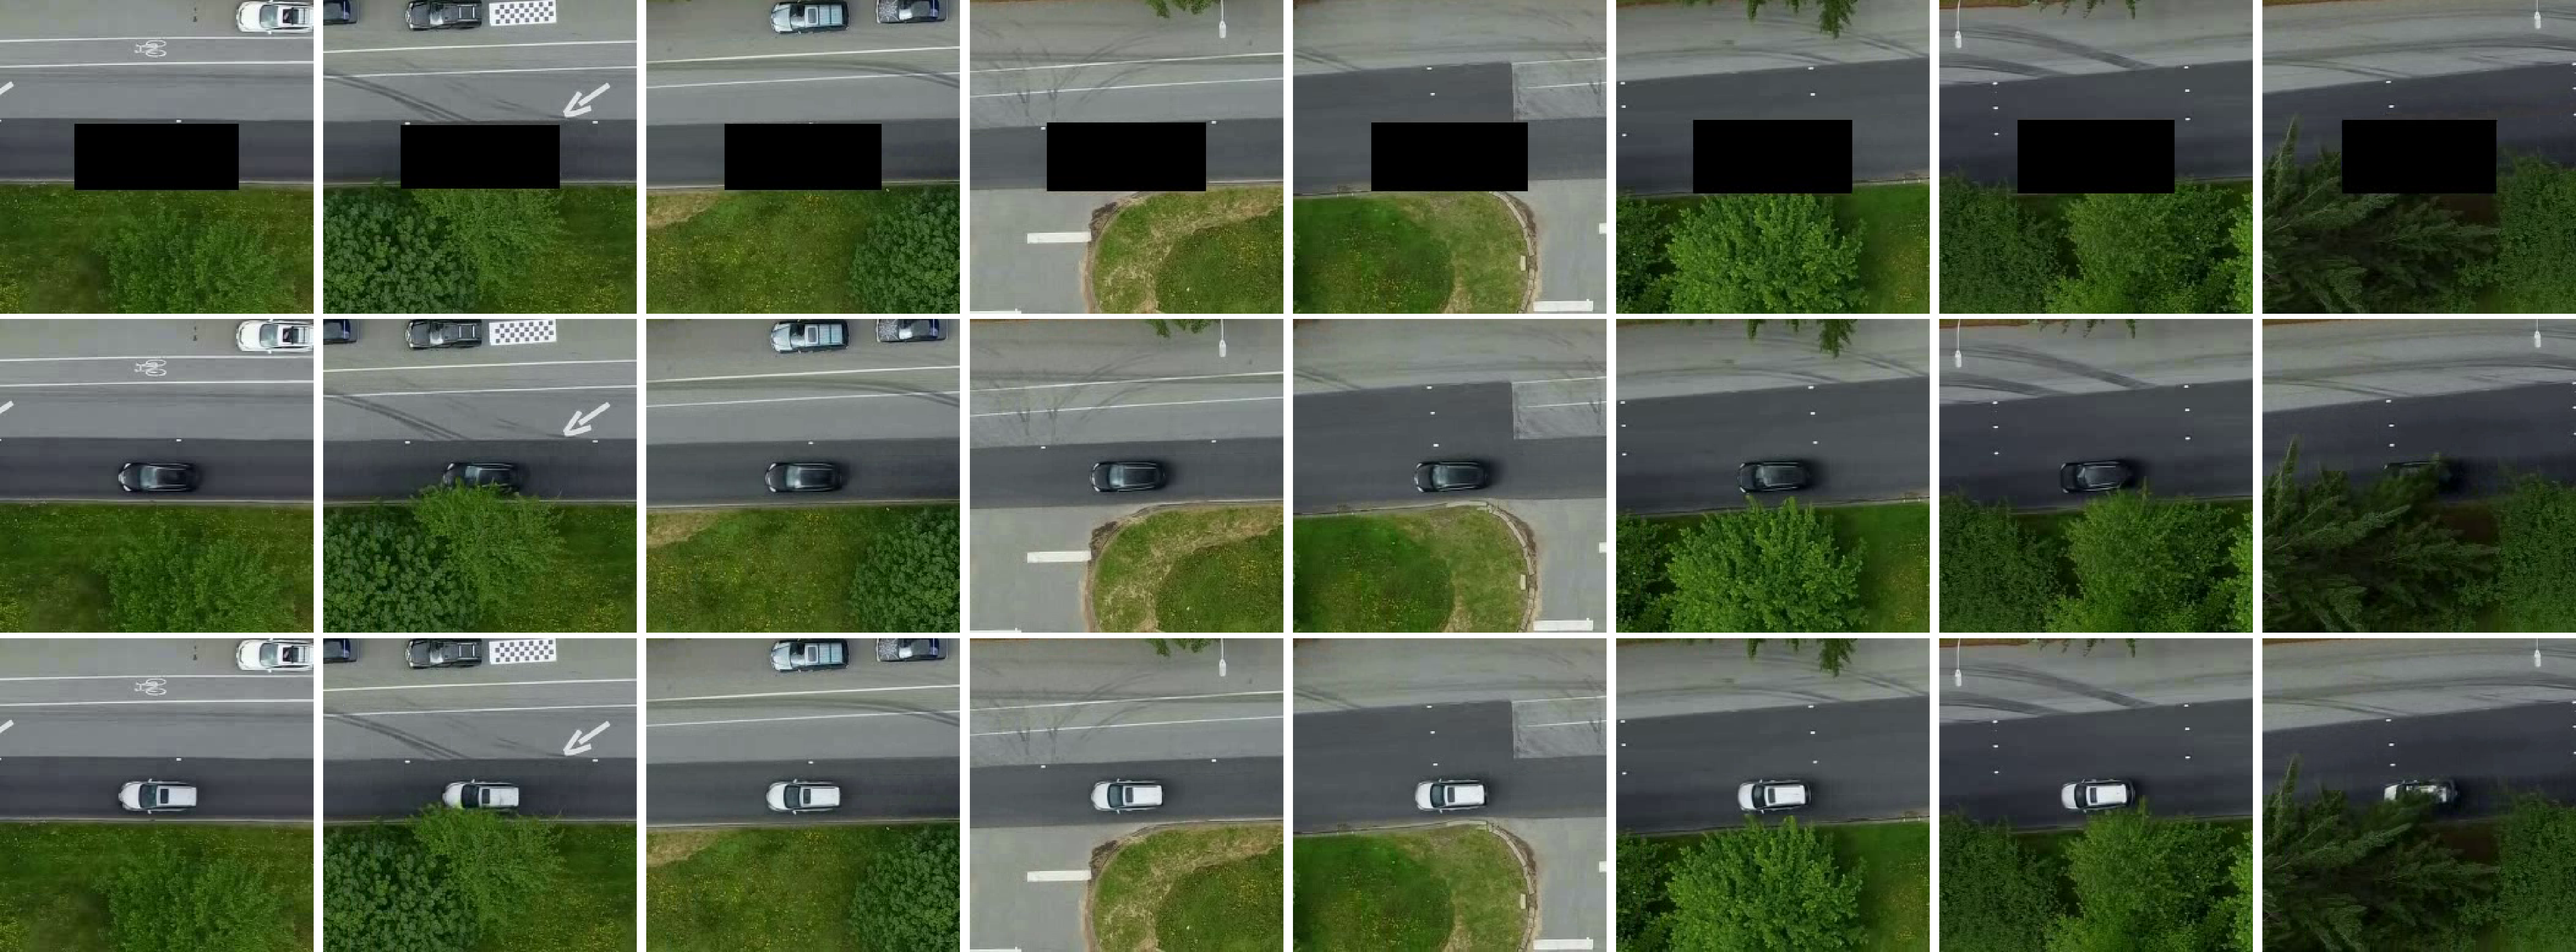
\includegraphics[width=\textwidth]{figures/additional-samples/cars_3028.pdf}
        \label{fig:extra-cars1}
    \end{subfigure}
    ~
    \begin{subfigure}[t]{\textwidth}
        \centering
        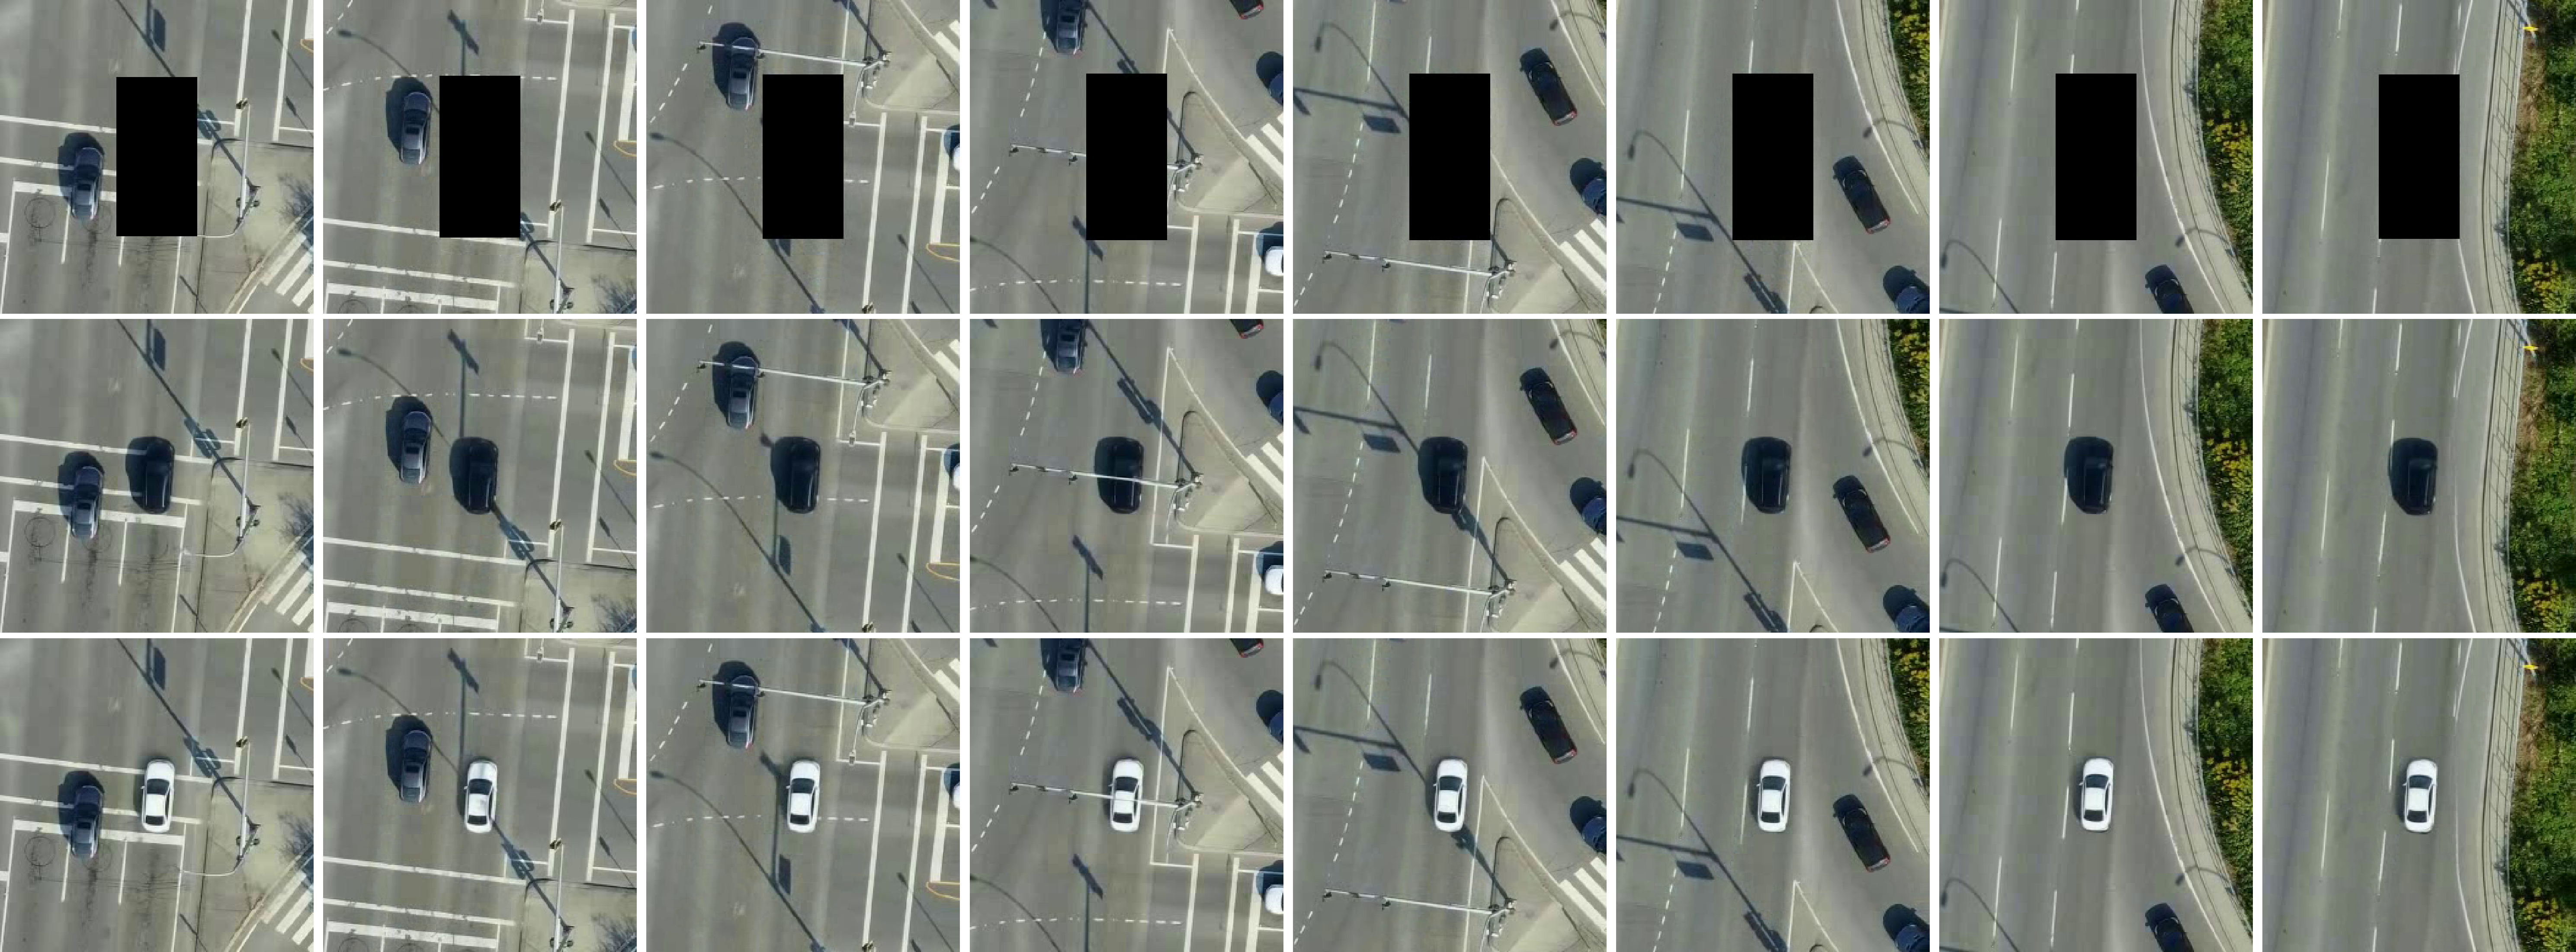
\includegraphics[width=\textwidth]{figures/additional-samples/cars_3067.pdf}
        \label{fig:extra-cars2}
    \end{subfigure}
    ~
    \begin{subfigure}[t]{\textwidth}
        \centering
        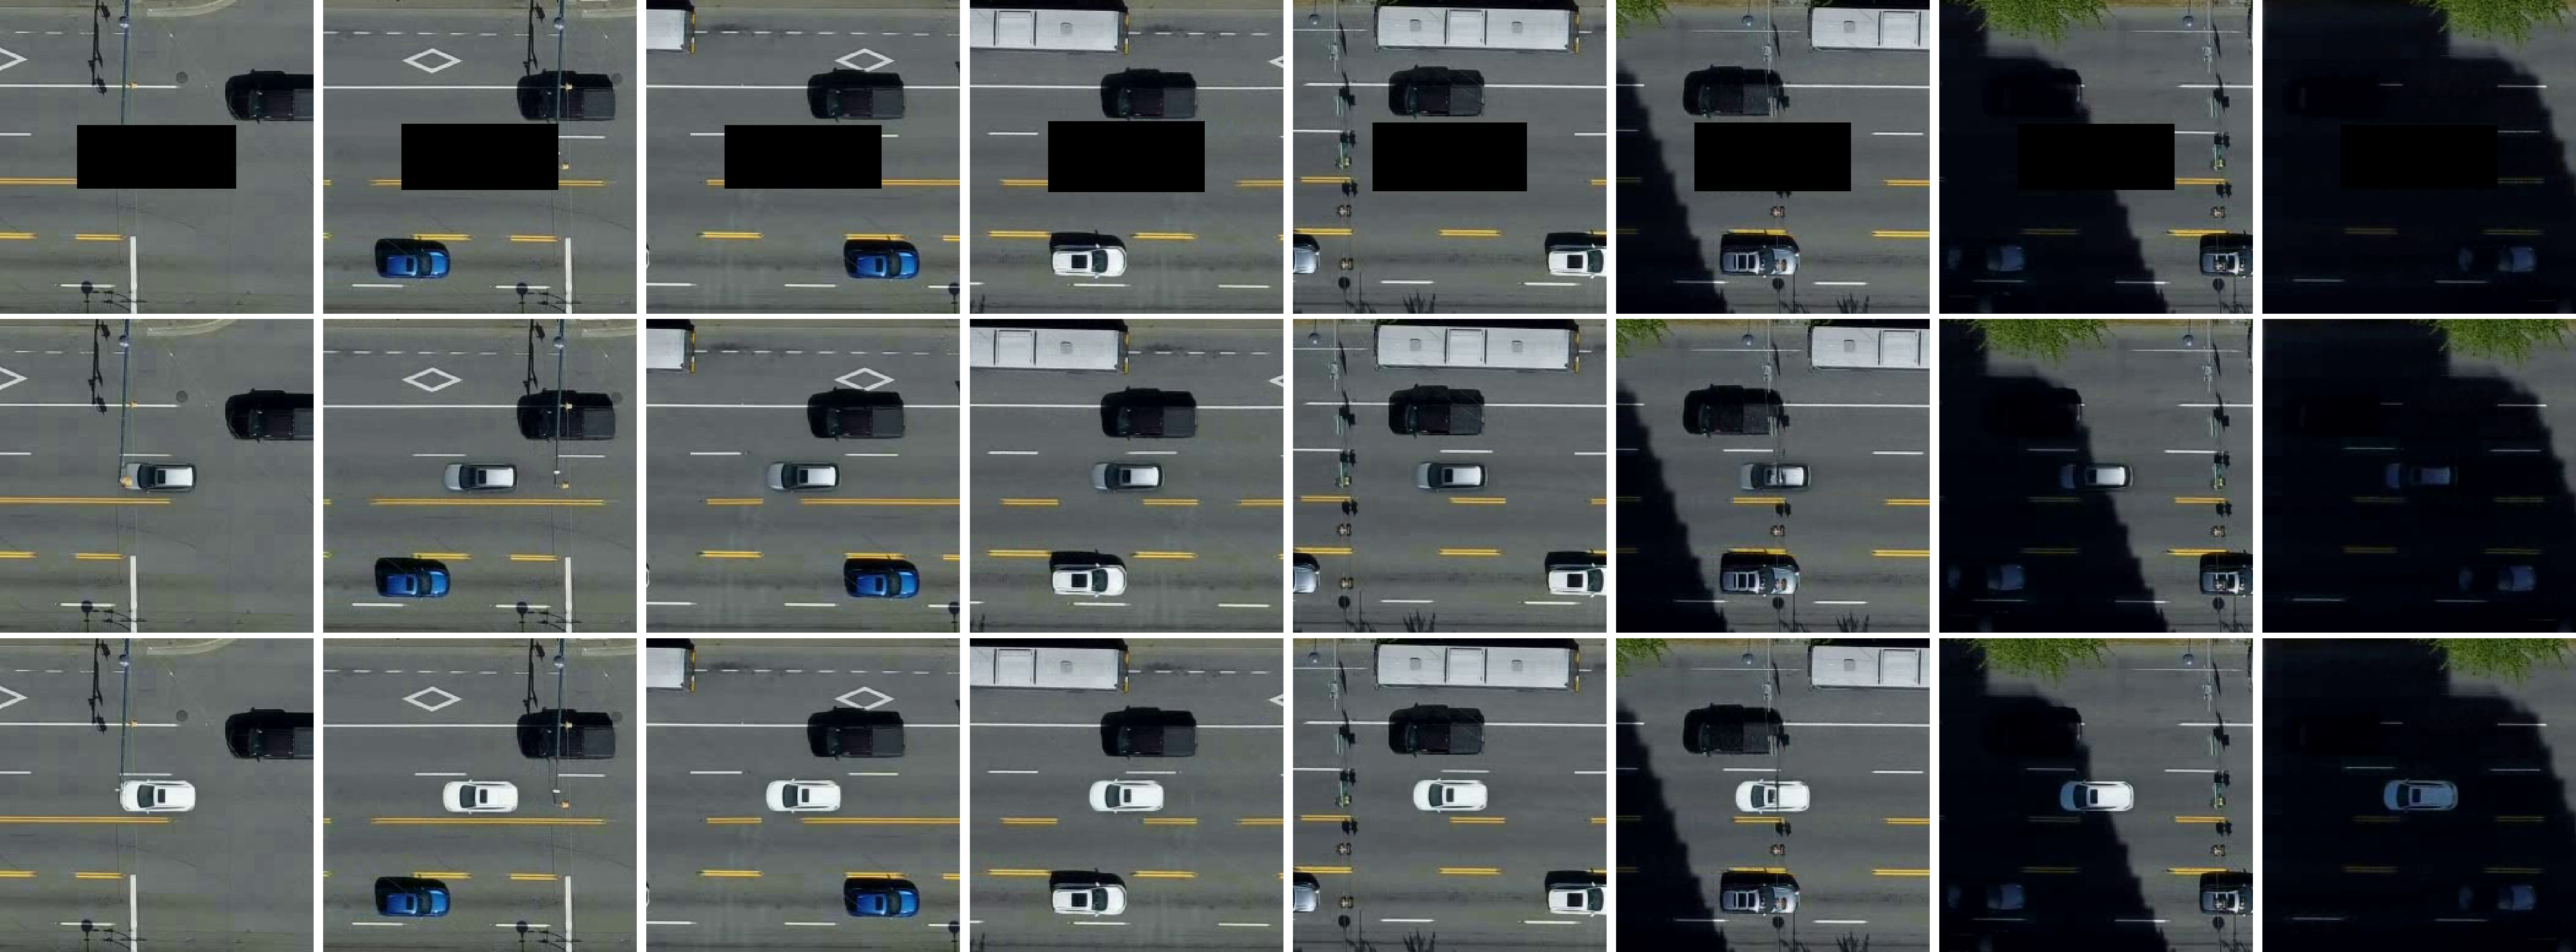
\includegraphics[width=\textwidth]{figures/additional-samples/cars_3093.pdf}
        \label{fig:extra-cars3}
    \end{subfigure}%
    \caption[Additional qualitative results from our method on the Inpainting-Cars
    test set.]{Additional qualitative results from our method on the Inpainting-Cars test set, demonstrating our method's ability to generate diverse vehicle appearances to inpaint the scene and to deal with various complications in the context.  In \Cref{fig:extra-cars1}, our method is able to deal with partial occlusion by trees in the scene. In \Cref{fig:extra-cars2}, note that the inpainted cars' shadows are oriented in the same direction as the shadows of other objects. \Cref{fig:extra-cars3} demonstrates that our method is capable of realistically shading an inpainted vehicle's color when it enters the shade.
    }
    \label{fig:extra-cars}
\end{figure}
